\documentclass[../main.tex]{subfiles}

\begin{document}

%%%%%%%%%%%%%%%%%%%%%%%%%%%%%%%%%%%%%%%%%%%%%%%%%%%%%%%%%%%%%%%%%%%%%%%%%%%%%%%

\section{Propuestos y resueltos}

%%%%%%%%%%%%%%%%%%%%%%%%%%%%%%%%%%%%%%%%%%%%%%%%%%%%%%%%%%%%%%%%%%%%

\begin{itemize}
    \item \textbf{Pregunta primera:}
\end{itemize}

 Dado $l$, encuentre la forma del potencial $U(r)$ tal que la trayectoria de una partícula sujeta a este potencial esta dado por la espiral $r(\phi)=r_0e^{\alpha \phi}$, donde $r_0$ y $\alpha$ son constantes. Discuta la física del sistema. \\
\\
\textbf{Solución:} Primero, para encontrar el potencial asociado a la fuerza central que experimenta una partícula que se mueve con la trayectoria $r(\phi)=r_0e^{\alpha \phi}$ es necesario calcular la fuerza central que experimenta esta partícula. 
\\
Primero, el enunciado nos menciona dado un $l$ el cual asumiremos constante, ya que, la trayectoria está expresada en coordenadas polares y su movimiento en la dirección $z$ es cero o constante. Luego, las ecuaciones de movimiento son
\begin{align}
    -\frac{l^2}{mr^2} \left( \frac{d^2}{d \phi^2}\left( \frac{1}{r}\right)+\frac{1}{r} \right) & =f(r) \\ 
    mr^2\dot{\phi} & =l  
\end{align}
La primera ecuación corresponde a la ecuación de Binet, con la cual se obtendrá la fuerza central, tal que:
\begin{align*}
    f(r) & =  -\frac{l^2}{mr^2} \left( \frac{d^2}{d \phi^2}\left( \frac{e^{-\alpha\phi}}{r_0}\right)+\frac{e^{-\alpha\phi}}{r_0} \right) \\
    & = -\frac{l^2}{mr^2} \left( \frac{\alpha^2e^{-\alpha\phi}}{r_0} + \frac{e^{-\alpha \phi}}{r_0} \right) \\
    & =  -\frac{l^2}{m} \frac{e^{-2\alpha \phi}}{r_0^2} \left( \frac{e^{-\alpha \phi}}{r_0}\left(\alpha^2+1 \right)  \right) \\
    & = -\frac{l^2}{m} \frac{e^{-3\alpha \phi}}{r_0^3}\left(\alpha^2 +1\right) \\
    & = -\frac{l^2(\alpha^2+1)}{m r^3}
\end{align*}
Con lo cual se obtiene una fuerza central del orden de la tercera potencia inversa $f(r)=-\frac{l^2(\alpha^2+1)}{m r^3}\hat{r}$, ahora, al ser una fuerza conservativa se busca un potencial que cumpla $\vec{f}(r)=-\vec{\nabla} U(r)$ o lo que es igual ${f}(r)=-\frac{\partial }{\partial r}U(r)$, con lo cual se procede a integrar, tal que:
\begin{align*}
    \int_{a}^r -\frac{l^2(\alpha^2+1)}{m r^3} & =-U(r)+{U(a)} \\
\end{align*}
Ahora si $\lim_{a \to \infty}U(a)=0$ queda tal que 
\begin{align*}
    -\frac{l^2(\alpha^2+1)}{2m r^2} & = U(r)
\end{align*}
Ahora, es correcto analizar la energía del sistema, con lo cual primero notamos que,
la energía del sistema está dada por:
\begin{equation}
    E=\frac{m \dot{r}^2}{2}+U_{eff}
\end{equation}
En la cual $U_{eff}$ corresponde al potencial efectivo dado por:
\begin{equation*}
    U_{eff}(r)= U(r)+ \frac{l^2}{2mr^2} 
\end{equation*}
Reemplazando el potencial obtenido $U(r)$ se obtiene:
\begin{align*}
    U_{eff}(r) & = -\frac{l^2(\alpha^2+1)}{2m r^2} + \frac{l^2}{2mr^2} \\
    & = -\frac{l^2\alpha^2}{2m r^2}
\end{align*}
Ahora, si se sigue analizando la energía, se tiene que, con el potencial efectivo es:
\begin{equation*}
    E= \frac{m \dot{r}^2}{2}-\frac{l^2\alpha^2}{2m r^2}
\end{equation*}
Para seguir operando es necesario encontrar una expresión para $\dot{r}$, con lo cual se tiene que:

\begin{equation*}
    \dot{r}=\frac{dr}{d\phi}\cdot \frac{d\phi}{dt}
\end{equation*}
con lo cual
\begin{equation*}
    \dot{r}=\alpha r_0 e^{\alpha \phi} \dot{\phi}
\end{equation*}
y recordemos que $\dot{\phi}=\frac{l}{mr^2}$ con lo cual $\dot{r}$ queda tal que:
\begin{equation}
    \dot{r}= \frac{\alpha l}{m r}
\end{equation}
Ahora reemplazando esto en la energía se tiene:
\begin{align*}
    E & = \frac{m}{2} \left( \frac{\alpha l}{m r} \right)^2-\frac{l^2\alpha^2}{2m r^2} \\
    & = \frac{l^2\alpha^2}{2mr^2}-\frac{l^2\alpha^2}{2m r^2} \\
    & = 0
\end{align*}
De ello se puede concluir que, para cualquier $r$ la energía del sistema sera siempre cero, $E=0$, lo cual ya da indicios de un movimiento con trayectoria abierta y no orbital. \\
De lo cual se puede notar que, al igual que la fuerza central obtenida $f(r)$ este potencial efectivo no dependerá del signo que tome la constante $\alpha$. Ya que el término se encuentra al cuadrado. El caso de $\alpha=0$ es un caso especial que se discutirá más adelante.
\begin{figure}[h]
    \centering
    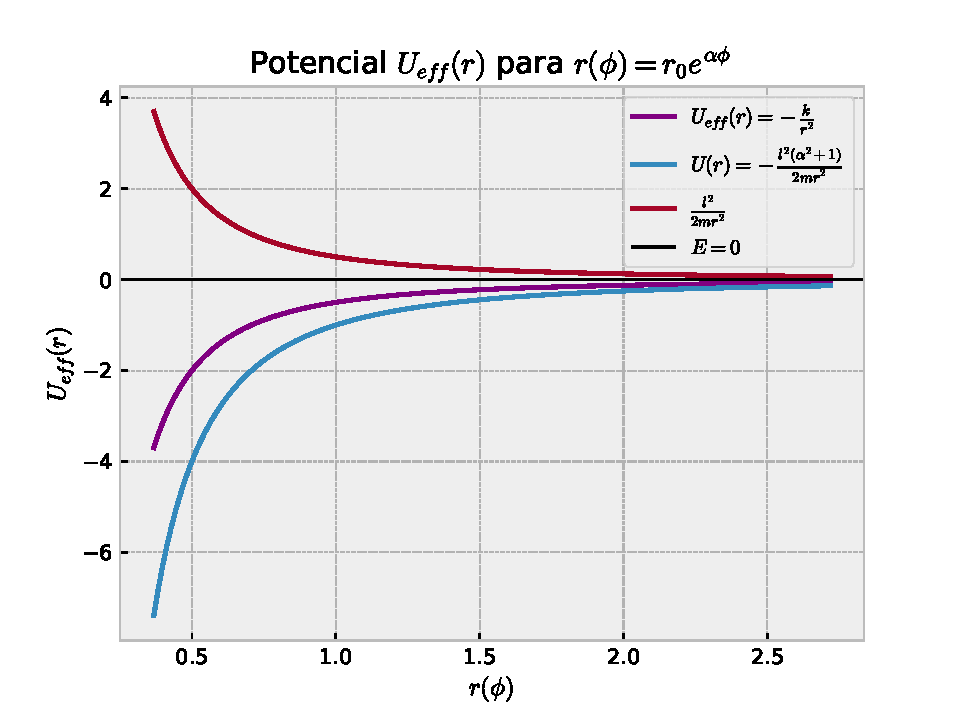
\includegraphics[scale=0.7]{img/fuerzas-centrales/potencial1.pdf}
    \caption{Potencial efectivo para una fuerza atractiva de la tercera inversa y alpha distindo de cero}
    \label{fig:1}
\end{figure}
En el se puede observar y notar de inmediato que la curva de $U_{eff}$ para el gráfico \ref{fig:1} es cóncava negativa y su máximo está en $y=0$ cuando $r\to \infty$, en este caso, el potencial . \\
También se puede observar que, sin importar el signo de $\alpha$, en el caso de $\alpha$ negativo, la forma del potencial efectivo no cambia cualitativamente, por tanto la física es la misma, lo que cambiará en este caso será la dinámica del sistema. Esto será abordado mas adelante.
\\
Ahora \textbf{¿Que sucede si alpha es cero?}, $\alpha=0$ presenta un caso límite en los apartados discutidos anteriormente, en el cual tenemos lo siguiente. Primero, con $\alpha=0$ el radio será $r(\phi)=r_0$ para cualquier $\phi$ y por tanto tenemos un radio constante, esto a simple vista sugiere una órbita circular.\\
Como $\alpha=0$ su energía no sera la misma, ya que:
$$U_{eff}(r)=-\frac{l^2\alpha^2}{2mr^2}=0$$
si su potencial efectivo es cero entonces su energía total dependerá solo de la energía cinética $T$, tal que:
\begin{align}
    E & =T \\
    & = \frac{m\dot{r}^2}{2}
\end{align}
Como el valor de $\dot{r}$ para un radio constante es cero entonces al igual que en los apartados anteriores
$$E=0$$
lo que puede significar que la partícula esta en reposo o en equilibrio para un radio constante $r_0$y se puede decir que, como no hay energía potencial ni cinética entonces la partícula no experimenta ningún tipo de fuerza central a menos que una condición inicial lo sugiera.

\textbf{Analicemos la física del sistema.} \\
Se tiene una fuerza que sigue una ley de la tercera inversa,
$$f(r)=-\frac{l^2(\alpha^2+1)}{m r^3}\hat{r}$$
Fuerza la cual es atractiva y depende tanto de las constantes de la trayectoria como de $l$. \\
Cuyo potencial sigue la ley de la segunda inversa negativa y es igual a
$$U(r)=-\frac{l^2(\alpha^2+1)}{2m r^2}$$
y cuyo potencial efectivo asociado es igual a
$$U_{eff}(r)=-\frac{l^2\alpha^2}{2m r^2}$$
Como se observa en el gráfico \ref{fig:1} el potencial efectivo alcanza es siempre negativa y monótona creciente independiente del signo de $\alpha$, con lo cual no tiene mínimos ni máximos locales, lo cual, junto a que es cóncava negativa, nos indica que no hay un radio mínimo en el sentido clásico de una barrera potencial, o sea, el potencial disminuye a medida que $r$ también lo hace, pero, la geometría del sistema nos indica que para $\alpha>0$ la partícula partirá de un radio inicial o mínimo $r_0$ cuando $\phi=0$ el cual ira creciendo, y a su vez, el potencial efectivo decreciendo en la segunda potencia inversa, luego, en el caso que $\alpha<0$ nos indica que la partícula inicia en un radio $r_0$ para luego decrecer y caer hacia el centro de fuerzas en forma de espiral para el cual $U_{eff}(r)\to \infty$ cuando $r(\phi)\to 0$.

Cabe destacar que, en el caso de que el radio tienda a infinito, es posible que la partícula alcance un punto de retorno en el infinito. Esto se debe a que el potencial efectivo decrece asintóticamente hacia cero a medida que $r$ tiende a infinito, sugiriendo que la partícula no escapará al infinito pero tampoco se quedará en una posición fija, sino que retornará eventualmente hacia valores de $r$ más pequeños. Esto refuerza la idea de que la trayectoria es abierta y no orbital.

La condición que la energía será cero nos indica de una trayectoria abierta, en este caso espiral, que mantiene sus valores de energía cinética $T$ y potencial efectivo $U_{eff}(r)$, de la forma $U_{eff}(r)=-T$, ambos los cuales tienden a cero cuando $r\to \infty$ y tienden a infinito cuando $r\to 0$ como sugiere el sistema, lo que nos indica que la partícula es tanto capaz como de escapar hacia el infinito como de quedar atrapada y colapsar en el centro de fuerzas para los casos planteados. \\

El caso límite entre estas dos dinámicas seria el de $\alpha=0$ en el cual la partícula ni se aleja ni se acerca al centro de fuerzas, sino que está en equilibrio a una distancia $r_0$, ya que su $E=0$ así lo sugiere.
\\
\\
Ahora, el \textbf{teorema de Bertrand} establece que solo los potenciales de la forma $-\frac{k}{r}$(Ley del inverso cuadrado) y $\frac{kr^2}{2}$(Ley de Hooke)
resultan en órbitas cerradas para cualquier condición inicial, pero, el potencial del problema es de la forma $-\frac{k}{r^2}$ el cual no cabe dentro de esta categoría. En consecuencia, no producirá órbitas cerradas y las trayectorias serán abiertas, en este caso, para cualquier $\alpha>0$ ó $ \alpha<0$ la trayectoria será abierta con un radio inicial $r_0$, y como el problema sugiere, de la forma $r(\phi)=r_0e^{\alpha \phi}$.\\
En resumen, de la dinámica del sistema se concluye que, dado que el potencial efectivo $U_{eff}(r)$ es siempre negativo, tiende a cero en el infinito, es cóncavo negativo y considerando que $E=0$, la partícula seguirá una trayectoria abierta y confirma la inexistencia de radios mínimos para el potencial, pero si radios mínimos para la trayectoria sugerida, siendo esto consistente con el teorema de Bertrand, el cual predice que este tipo de potencial no produce órbitas cerradas. También, se ha concluido que para el caso especial de $\alpha=0$ el sistema se quedará en equilibrio a una distancia $r_0$ sin energía, fuerzas ni potencial presentes.

\end{document}